\section{Hwang \& Lee (2007): Database of Rotating Cluster}
Hwang and Lee used redshift and position angle of galaxies to estimate the ratio of cluster rotation amplitude to dispersion and the velocity gradient across the clusters. They took 899 Abell clusters as their sample clusters.\\\\
Methods for identification of the rotating cluster candidates:
\begin{itemize}
\item To select member galaxies in target cluster they used \textquoteleft shifting gapper\textquoteright\,\, by Fadda et al. (1996). They selected 56 clusters in which the number of the galaxies is greater than or equal to 40.
\item To investigate the global rotation property of galaxy the observed radial velocity $v_p$ of the cluster galaxies is fitted with function of position angle $$v_p(\Theta)=v_{sys}+v_{rot}\;sin(\Theta-\Theta_0)$$ where $\Theta$ is projected position angle of galaxy relative to the cluster center (measured from north east), $\Theta_0$ is the projected postion angle of the rotation axis of the cluster, $v_{rot}$ is the systemic velocity of the galaxy clusters.\\\\
Similarly, the effect of global rotation of galaxy clusters also can appear as velocity gradient. They fit the observed radial velocity gradient of the cluster galaxies with a function of a position in the plane of sky.
$$
	v_p(x,y)=v_{sys}+\frac{\partial v}{\partial X}X+\frac{\partial v}{\partial Y}Y
$$ where $X$ and $Y$  are clusteric centric distance in the direction of right ascession and declination respectively. They fitted the observed radial velocities of cluster galaxies with $v_{sys}$ as a fixed value of the mean radial velocity of the cluster galaxies.\\\\
A plot of velocity dispersion of galaxy cluster as a function of $\frac{|v_{rot}|}{\sigma_p}$ and as a function of $\frac{dv}{dR}=\sqrt{\left(\frac{dv}{dx}\right)^2+\left(\frac{dv}{dy}\right)^2}$ was drawn. The rotating cluster has large ratio of the absolute velocity dispersion and has large velocity gradient across the cluster. So, among 56 clusters they selected 12 rotating clusters whose $|\frac{v_{rot}}{\sigma_p}|>0.53$ and $\frac{dv}{dR}>380$ km\,s$^{-1}$\,Mpc$^{-1}$.
\end{itemize}

\begin{table*}
\caption[]{Database of three rotating clusters. First three columns
list the Abell name and positions of the cluster center as given
in ACO catalog (Abell et al. 1989). The next three columns give
cluster morphology (BM type classification, Bautz \& Morgan 1970),
mean radial velocity ($cz$ km\,s$^{-1}$) of the cluster and velocity dispersion
($\sigma_{\rm P}$ km\,s$^{-1}$) as given in Hwang \& Lee  (2007). The last
three columns give the number (N) of galaxies with known
diameters,  cluster diameters (arcmin) (Abell et al. 1989) and X-ray
luminosity (10$^{44}$\,erg\,cm$^{-2}$\,s$^{-1}$) (Ledlow et al. 2003, Bohringer et al. 2004).}
$$
 \begin{array}{lllllllll}
            \hline
            \noalign{\smallskip}
            $Cluster$  &  $R.A.$     & $Dec.$     &  $BM-type$ &  $cz$  &  \sigma_{\rm p}     &  $N$  &  $$a$$ & L_{x}\\
             \noalign{\smallskip}
            \hline
            \noalign{\smallskip}
            A1139    &   10^{\rm h}58^{\rm m}10.39^{\rm s}   &   01^{\circ}35'11.0'' &   $III$    &   11\,849   &   491    &   121 & 70  &  0.09  \\
            A2162    &   16^{\rm h}12^{\rm m}30.00^{\rm s}   &   29^{\circ}32'23.0'' &   $II-III$ &   9\,653    &   416    &   41  & 356  &  0.01  \\
            A2366    &   21^{\rm h}42^{\rm m}50.41^{\rm s}   &   06^{\circ}52'15.0'' &   $I-II$   &   15\,914   &   604    &   41  & 40  &  0.05  \\
            \noalign{\smallskip}
            \hline
         \end{array}
     $$
\end{table*}


\begin{figure}[H]
\centering 
\centering
   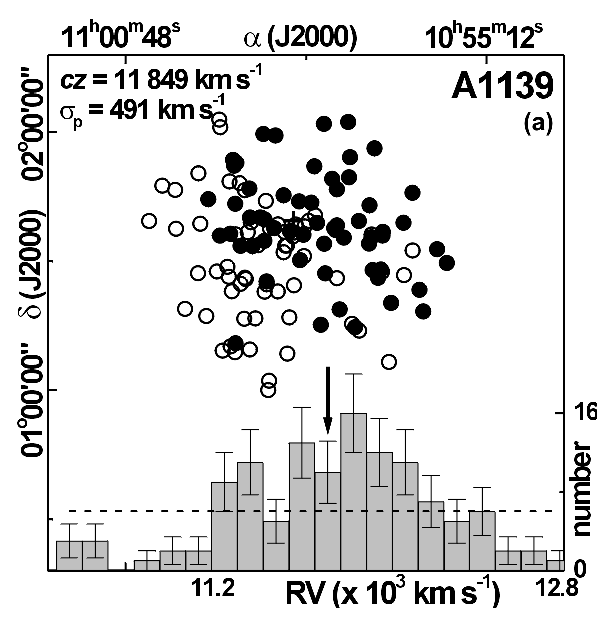
\includegraphics[height=6.0cm]{fig3a.eps}
   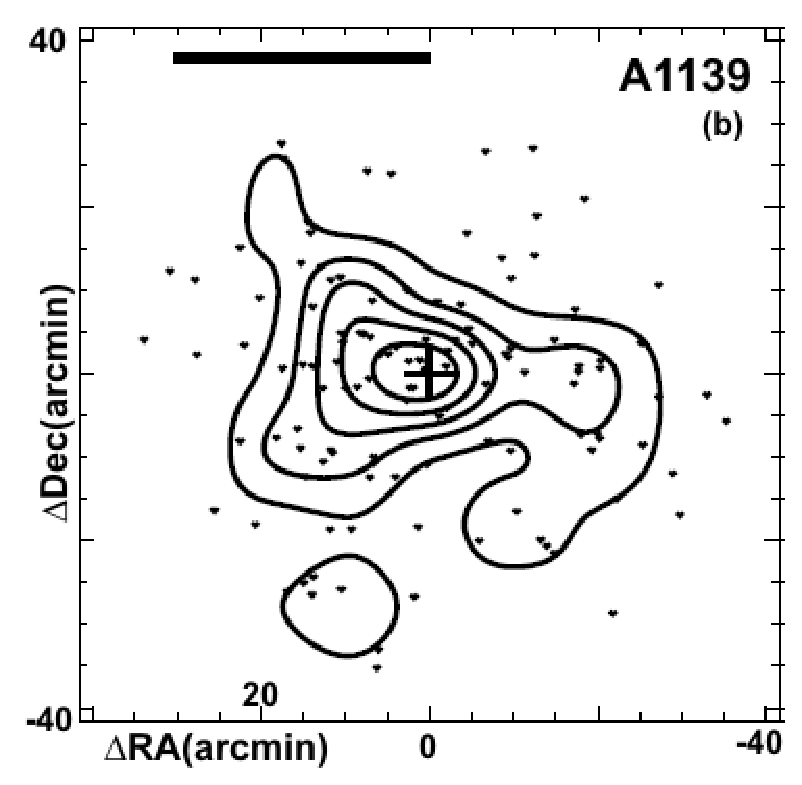
\includegraphics[height=6.0cm]{fig3b.eps}\\
   \includegraphics[height=6.5cm]{gal_a1139.eps}
   \includegraphics[height=6.5cm]{sup_a1139.eps}
   \caption{(a) All sky distribution of galaxies in the cluster A1139. The solid (hollow) circle represents the galaxies that have radial velocity less (greater) than
      the mean radial velocity ($cz$) of the cluster. The histogram showing RV distribution of galaxies can be seen.
      The dashed line and an arrow represent the average distribution and the cluster mean radial velocity ($cz$).
      (b) Galaxy number density map. The member galaxies are represented by dots, and the number density contours are overlaid.
      The cross indicates the cluster center, and the thick horizontal bar represents the physical size of 1 Mpc.
    (c) All sky distribution of the galaxies in galactic coordinate system. (d) All sky distribution of galaxies in the Supergalactic coordinate system.}
\end{figure}
\begin{figure}[H]
\centering
      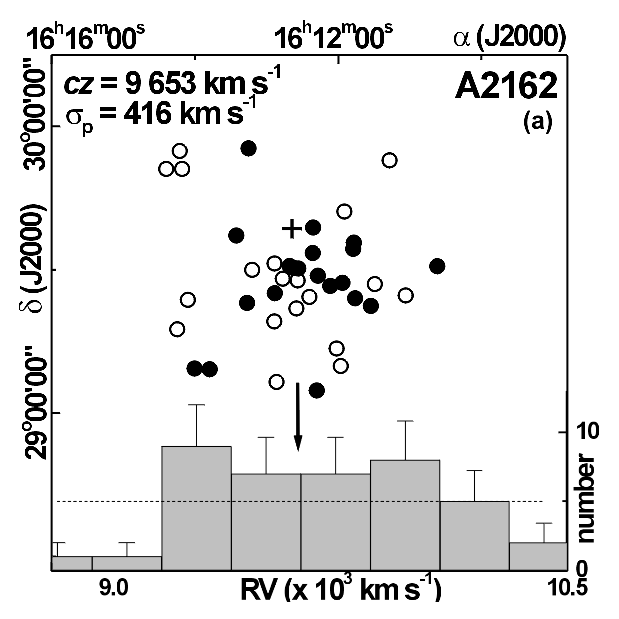
\includegraphics[height=6.0cm]{fig5a.eps}
   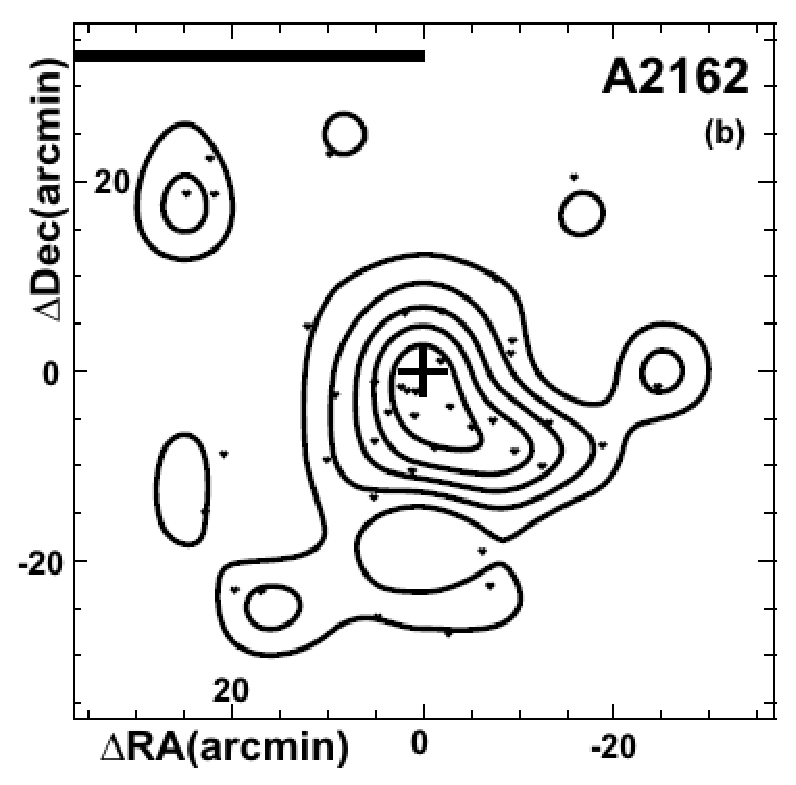
\includegraphics[height=6.0cm]{fig5b.eps}\\
    \includegraphics[height=6.5cm]{gal_a2162.eps}
   \includegraphics[height=6.5cm]{sup_a2162.eps}
   \caption{(a) All sky distribution of galaxies in the cluster A2162. The solid (hollow) circle represents the galaxies that have radial velocity less (greater) than
      the mean radial velocity ($cz$) of the cluster. The histogram showing RV distribution of galaxies can be seen.
      The dashed line and an arrow represent the average distribution and the cluster mean radial velocity ($cz$).
      (b) Galaxy number density map. The member galaxies are represented by dots, and the number density contours are overlaid.
      The cross indicates the cluster center, and the thick horizontal bar represents the physical size of 1 Mpc.
    (c) All sky distribution of the galaxies in galactic coordinate system. (d) All sky distribution of galaxies in the Supergalactic coordinate system.}
\end{figure}
\begin{figure}[H]
\centering
   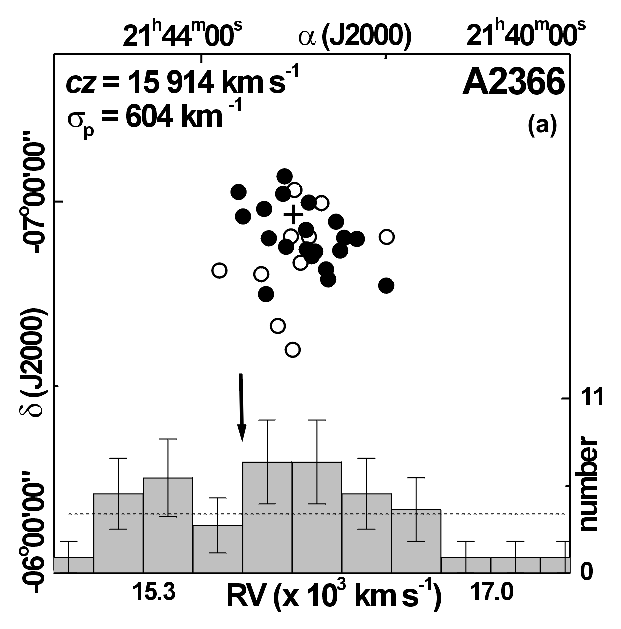
\includegraphics[height=6.1cm]{fig7a.eps}
   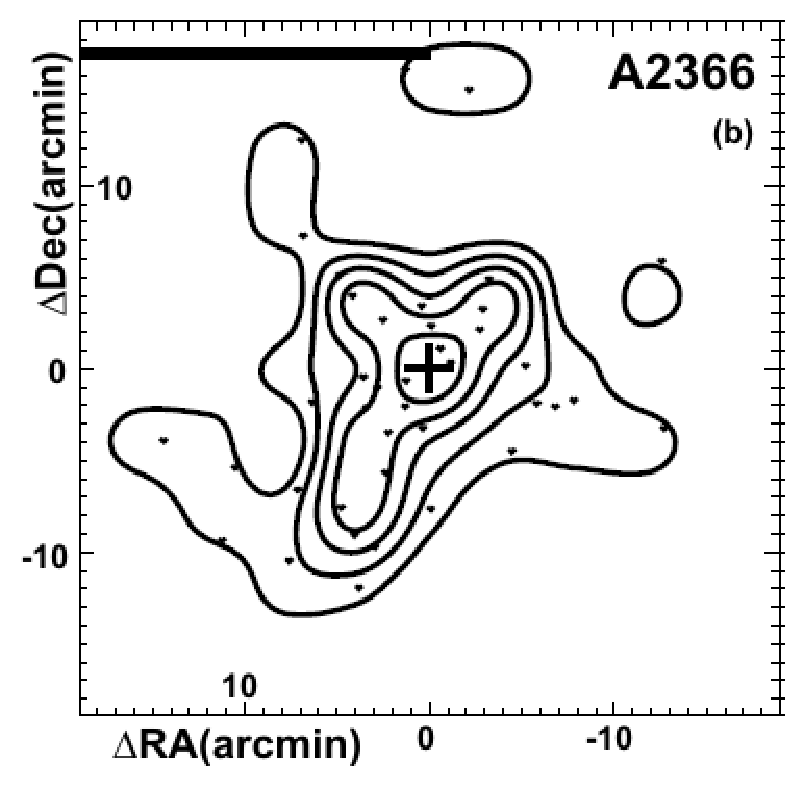
\includegraphics[height=6.0cm]{fig7b.eps}\\
    \includegraphics[height=6.5cm]{gal_a2366.eps}
   \includegraphics[height=6.5cm]{sup_a2366.eps}
   \caption{(a) All sky distribution of galaxies in the cluster A2366. The solid (hollow) circle represents the galaxies that have radial velocity less (greater) than
      the mean radial velocity ($cz$) of the cluster. The histogram showing RV distribution of galaxies can be seen.
      The dashed line and an arrow represent the average distribution and the cluster mean radial velocity ($cz$).
      (b) Galaxy number density map. The member galaxies are represented by dots, and the number density contours are overlaid.
      The cross indicates the cluster center, and the thick horizontal bar represents the physical size of 1 Mpc.
    (c) All sky distribution of the galaxies in galactic coordinate system. (d) All sky distribution of galaxies in the Supergalactic coordinate system.}
\end{figure}
